\documentclass[11pt]{article}
\usepackage{times}
\usepackage[dvips]{graphicx}
\usepackage{latexsym,fullpage,amsmath,listings}
%\usepackage{latexsym,fullpage,times}
\usepackage{float,array}
\usepackage[colorlinks]{hyperref}

\begin{document}

\begin{center}
{\Large ME/IE/CS 558}\\
\vspace{12pt}
{\large Assignment 4}\\
\vspace{12pt}
{\em Due April 13, 2018}
\end{center}

{\bf For all assignments:}
{\em Unless specifically indicated,  you are free to use any
publicly available sources: papers, books, programs, online
material, etc. -- as long as you clearly indicate and attribute
the origin of the information.}


\vspace{24pt}
The goal of these assignment is to modify your program for 
computing Delaunay triangulation
(Assignment 3) to compute the Voronoi diagram for a (triangulated)
set of points (sites) $P$,  and to use it for the problem of 2D
curve reconstruction.   You may find 
Exercise 5.7.5(2) on page 189 in the O'Rourke's book helpful.

\begin{enumerate}

\item Analysis (50 points)
\begin{enumerate}

\item
Describe modifications (if any) to your data structures for Delaunay
triangulation and give a high-level description of the algorithm to
compute  (and draw)  the Voronoi diagram.   In order to deal with   the Voronoi edges 
that go off to infinity, enclose your triangulation into a (much larger) box (or disk, 
or triangle);  instead of points at infinity,  you can now store the points of
intersection between the Voronoi edge and the enclosing box.  


\item 
Recall the idea of the ``crust algorithm'' for shape reconstruction. 
First construct a Delaunay triangulation of input points;  then 
add the centers of circumcircles and recompute DT.  If the Delaunay edges 
appear in both triangulations, they are deemed to be good candidates
for boundary of the reconstructed shape.

\item
Recall that the Voronoi and Delaunay edges are dual to each other.  This means 
that for every edge in your data structure,  you actually have a choice of 
which edge to draw.   Let $a,b$ be the end points of the Delaunay edge, and 
$p, q$ are the end points of the corresponding (dual) Voronoi edge.  
Consider a drawing   procedure \emph{Shape} that  operates as follows:   if there 
exists a circle through points $a$ and $b$ that does not include the points $p$ 
and $q$,  then draw the Delaunay edge;  else draw the dual Voronoi edge.  Design an 
efficient procedure to perform this test. Compare  the result of this 
procedure and the output you expect to obtain from the ``crust algorithm''
outlined above. Are the Delaunay edges produced by the \emph{Shape} procedure and edges
produced by ``crust algorithm'' different or the same, and why?


% \item 
% Now consider the Voronoi edges produced by the \emph{Shape} procedure.  
% Explain whether or not they are allowed to intersect the Delaunay edges 
% produced by \emph{Shape} and why.  


\end{enumerate}

\item Implementation \& Testing (50 points)

\begin{enumerate}

\item 
Implement the program to produce a graphic output showing the computed Voronoi diagram.

\item 
Implement the program for the ``crust algorithm'' from the analysis portion 
of the homework.

\item
Test both programs on the same data you used to test your Delaunay triangulation program

\item
Test the ``crust algorithm'' on the points generated by on some closed curve.
You can create the curve by inputing the ordered list of points,  or generate 
points using parametric description of the curve.  How well do the Delaunay edges 
reconstruct the curve? A good source of planar parameteric curves is 
\href{http://mathworld.wolfram.com/topics/PlaneCurves.html}{http://mathworld.wolfram.com/topics/PlaneCurves.html}

\item
For voronoi diagram part, your program will be called from command line as
\begin{lstlisting}
>> python voronoi.py filename
\end{lstlisting}

Coordinates file stores n 2D points with the below format.

\begin{lstlisting}
x1 y1
x2 y2
...
xn yn
\end{lstlisting}

For example, for the following points.txt file, 
the below voronoi diagram should be plotted. (see Figure \ref{fig:voronoi}).

\begin{lstlisting}
4.607333	2.922295
3.625414	2.482151
0.958715	4.738811
2.560862	4.123219
3.790999	1.256218
3.977649	0.720602
2.253004	1.448505
4.673365	2.729893
0.392271	4.314042
0.112320	1.977590
\end{lstlisting}

\begin{figure}[H]
  \centering
  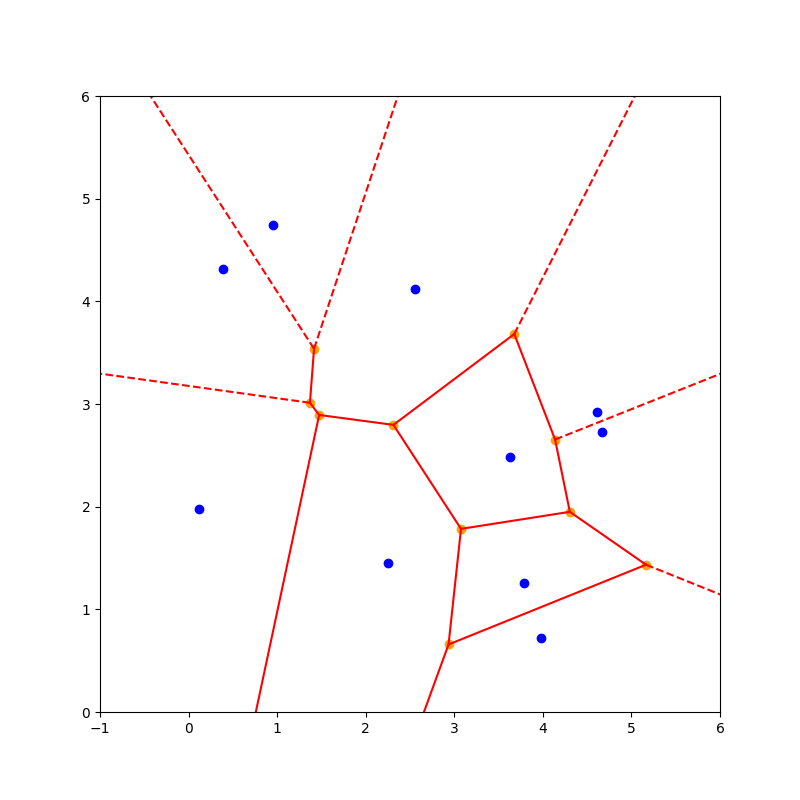
\includegraphics[scale=0.4]{points-1.png}
  \caption{Voronoi Diagram}
  \label{fig:voronoi}
\end{figure}

For ``crust algorithm'' part, your program will be called from command line as
\begin{lstlisting}
>> python crust.py filename
\end{lstlisting}

Coordinates file stores n 2D points with the below format.

\begin{lstlisting}
x1 y1
x2 y2
...
xn yn
\end{lstlisting}
For example, for sample points on a circle, ``crust algorithm`` should reconstruct the circle.
(see Figure \ref{fig:crust}).

\begin{figure}[H]
  \centering
  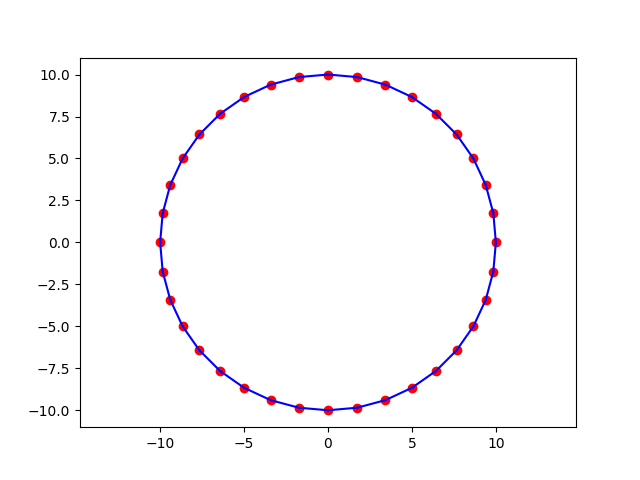
\includegraphics[scale=0.5]{crust.png}
  \caption{Crust Algorithm}
  \label{fig:crust}
\end{figure}

\end{enumerate}


\item Extra Credit (up to 15 points)
\begin{enumerate}
\item
Implement the program for the \emph{Shape} procedure from the analysis portion 
of the homework.
\item
Test the \emph{Shape} procedure on the points generated by on some closed curve.
You can create the curve by inputing the ordered list of points,  or generate 
points using parametric description of the curve.  How well do the Delaunay edges 
reconstruct the curve?   Speculate on the significance of the Voronoi edges 
produced by your procedure. 

\end{enumerate}


\end{enumerate}



\section*{Deliverables}

Please use the course website to submit a single  zip  named   FirstName\_LastName\_HW4.zip
The zip archive should contain:  (1) the analysis portion of the assignment,  (2)  the documented python source file, and (3) a PDF readme file  specfying the instructions for running the code.  It should also include at least 1 sample run with input and output,  and specify any specific dependencies or requirements of your code.  


\end{document} 
